\documentclass[acmlarge, screen, nonacm, 11pt]{acmart}
\usepackage[utf8]{inputenc}
\usepackage{float}
\usepackage{setspace}
\usepackage{pgfplots}
\usepackage{graphicx}
\usepackage{fancyvrb}
\usepackage{listings}
\usepackage[absolute]{textpos}\TPGrid{16}{16}
\usepackage{tikz}
  \usetikzlibrary{shapes}
  \usetikzlibrary{arrows.meta}
  \usetikzlibrary{arrows}
  \usetikzlibrary{shadows}
  \usetikzlibrary{trees}
  \usetikzlibrary{fit}
  \usetikzlibrary{calc}
  \usetikzlibrary{positioning}
  \usetikzlibrary{decorations.pathmorphing}
\usepackage{./tikz-uml}
\usepackage{xcolor}
\usepackage{hyperref}
  \hypersetup{colorlinks=true,allcolors=blue!40!black}
\setlength{\topskip}{6pt}
\setlength{\parindent}{0pt} % indent first line
\setlength{\parskip}{6pt} % before par
\date{\small\today}
\title[DeGit white paper]{[DRAFT] White-paper: DeGit - distributed git repository manager}
\definecolor{tikz-block}{HTML}{232527}
\tikzset{node distance=1.6cm, auto, every text node part/.style={align=center, font={\sffamily\small}}}
\tikzstyle{block} = [draw=tikz-block, fill=white, inner sep=0.3cm, outer sep=0.1cm, thick]
\tikzstyle{ln} = [draw, ->, very thick, arrows={-triangle 90}, every text node part/.append style={font={\sffamily\scriptsize}}]
\tikzstyle{O} = [circle, draw, every text node part/.style={align=center, font={\sffamily\small}}]

% custom commands
\newcommand{\code}[1]{\texttt{#1}}
\newcommand{\todo}[1]{\textcolor{red}{TODO: #1}}

\author{Kirill Chernyavskiy}
\email{g4s8.public@gmail.com}

\acmBooktitle{none}
\acmConference{none}
\editor{none}

\begin{document}
\raggedbottom

\begin{abstract}
  DeGitX is a distributed git repository manager.
  It provides a front-end interface for git operations by
  exposing one of the supported endpoints for git clients, and
  hides the distributed nature of git storage located on back-end nodes.
  The back-end keeps git repository replicas simultaneously on
  multiple different nodes to scale up the read capacity,
  increase durability and provides better availability, especially
  for different geographically distributed regions.
\end{abstract}

\maketitle

\section{Introduction}\label{sec:intro}

Providing efficient access to code repositories is a significant challenge
that large software companies or open-source communities may face when
the number of code repositories used by software developers counts
on millions. This challenge becomes especially critical for companies
that have distributed teams around the world.  In this case, using a single
git server does not provide even nearly-appropriate performance.
On the other hand, deploying multiple servers with load balancing is likewise not feasible
because storage I/O scaling is not possible for reading operations.

This article describes how to achieve significant performance improvement
by configuring a distributed git repository storage that replicates
repositories across nodes. The result can be achieved by implementing
a distributed Git repository manager DeGit with strong-consistent replica
nodes, guaranteeing high availability for read operations,
as well as availability across different regions.
Such a solution also provides durability by replicating repositories
on different server racks and read scalability by routing fetch traffc
to different nodes.
There is a number of technical problems related to scalability,
dispatching, and consistency that need to be solved when implementing
the distributed Git repository manager with strong-consistent replica nodes.
In addition to describing the suggested solution's major work principles
and functionality, this article also addresses these issues.
The DeGit architecture and components, including the main system protocols
that enable the system to identify the node, establish the node's connection,
lookup at the node’s real address, and map a git repository to the
storage node, are also explained.
The potential presence of malicious nodes can misroute, corrupt,
or drop messages and routing information in the system.
This article reviews the security-related methods with which the adopted DeGit approach
uses to protect the system infrastructure from potential attacks.
In this paper, you can find detailed instructions on creating a new repository.
The article also explains how a node finds a replica with a git repository
and provides descriptions of the node discovery workflow and metadata
exchange components.
In this solution, the git communicates with the data storage via a front-end.
The document describes communication between the git and the front-end
and explains how data is passed between the front-end and the repository.
The functional and non-functional requirements for building a distributed
git repository storage and the metrics expected for large enterprises
are addressed further in the document. Readers can also find helpful
information regarding the comparison of DeGit with other solutions.

\section{Technical problems}\label{sec:technical-problems}

There are three main problems to solve for the distributed git repository manager (DGRM):
\begin{description}
\item[scalability] --- one repository may be used actively by many users simultaneously. Storage disk
  has input-output (IO) operation limits and cannot perform a lot of \code{fetch} operations in
  a short period of time. The git repository storage should be replicated on different system nodes to
  solve this problem.
\item[dispatching] --- the user does not know the network addresses of git repository storages. Also, according to the
  previous problem, one repository can be located on multiple replicas.
  Hence, the system should be able to locate and redirect the user's requests
  from git client\footnote{Git client is a software that performs git fetch and push operations; it can be
  a command-line tool, IDE or any graphical user interface communicating with DGRM} to correct git repository
  storage. It should lookup repository nodes in the system and load-balance requests to different storage replicas.
\item[consistency] --- the user may \code{push} to the repository and \code{fetch} then; in that case it must receive
  the same or newer data that user \code{push}ed previously, even if the user \code{fetch}ed data from another
  replica of this repository. The linearizability of every single repository in a system is a must-have option.
\end{description}

\subsection{Scalability}\label{sec:scalability}

Big software companies or large developer communities have
millions of repositories distributed around the world and big teams located in different countries
(regions). On a high load of \code{fetch} requests, git repository storage disks may go above IO operation limits.
Usually, repositories are accessed by different ways:
\begin{description}
  \item[Developer personal activity] --- programmers access git repositories via
    \code{git} client and performs \code{fetch}/\code{push} actions. Also, they
    may use web UI interface to upload files, edit files in browser, merge pull requests, etc.
    The number of requests for this activity is not very large, according to statistics.
  \item[API access] --- many services depend on repository management services: API robots
    collecting developers' activity, background code analyzers of a repository, IDEs communicating
    with repositories and reading some history data. The number of such requests is approximately
    a few thousand requests per minute for each million repositories.
  \item[CI systems] --- many events may trigger a CI workflow; most common events are:
    new commit pushed, new pull (merge) request created, new tag pushed, etc.
    On each action, the CI system downloads the whole repository to run some workflows,
    the download (\code{clone}) operation it typically accompanied by huge bandwidth consumption.
    In addition, some repositories may include submodules; this leads to submodules cloning by the CI
    system. According to statistics, the number of such operations is on the scale of ten thousand requests per minute
    for each million repositories.
\end{description}

Even in cases when git repository storage is distributed, and clients are routed to storage with the correct git repository,
a large amount of \code{fetch} traffic for one repository still able to
make disk go above input-output operations (IOP) limits, and repository storage will stop
serving requests.

Asynchronous replication of git repository data was one approach attempting to address such scalability problems;
the DGRM was a proof-of-concept, which aimed to eventually consistently guarantee that one repository was replicated 
asynchronously after any update operation to multiple git repository storages. Thererfore,
clients were load balanced to different git repository storages.
However, it did not succeed because of two reasons:
\begin{enumerate}
  \item fetch traffic was correlated with push frequency because of the huge amount of
  CI systems and API robots involved in the development process: each update event usually triggers
  a CI build immediately, and CI clones the repository. CI was able to clone only the
  primary repository (repository with actual data) because the replication has not been completed
  before CI cloning started.
  \item \code{push} and \code{fetch} frequency was not distributed uniformly over time --- in each
  repository team members may have different responsibilities for the review and merge process, while
  the project technical lead can merge all approved pull-requests in a short period of time
  which causes frequent push operations in a git repo.
\end{enumerate}

These two conditions lead to high fetch traffic peaks for git repositories:
Frequent push operations turn replication storages into an inconsistent state,
and lead to high fetch traffic to primary repository storages from CI systems, which clones these repositories.
This causes the same problems as were common for non-replicated system --- the primary node goes beyond IOPS limits and
rejects new \code{fetcj} requests.

Furthermore, \code{merge} is not the only way to ``update'' the repository. Many of other activities can do that as well,
such as:

\begin{description}
  \item[branches changing] \verb|create|/\verb|delete|/\verb|update| branches by git push or by using web page.
  \item[tags changing] \verb|create|/\verb|delete|/\verb|update| tags by git push or by releasing new version on web page.
  \item[special refs changing] when new merge request is created, a new\\
    \emph{\code{refs/merge-requests/IID\footnote{Internal id of a project on gitlab}/head}} named ref
    is created. When source branch of the merge request is updated, the ref is also updated.
  \item[migrations] sometimes repository administrator can migrate the repository to
    another physical device or another region node; it also could be treated as an update.
    Also, deleting a repository could be treated as migrating it to a trash area.
\end{description}

\subsection{Dispatching}\label{sec:dispatching}

Git client does not know where a repository replica is located in the system. The dispatching algorithm
should be able to locate the correct storage nodes (distributed system nodes) of the repository and redirect
each client's request to one of these nodes. Moreover, it is not enough just to redirect the client's request.
The dispatching endpoint should load-balance all requests for each particular repository to distribute
storage load over time. Round-robin load-balancing solves this problem since the scalability problems
occur only on peaks of high read traffic. Hence, statistically redirecting each next read request to
a different storage node reduces disk load by \code{n}-times, where \code{n} is the number of storage replicas.

\subsection{Consistency}

\todo{Describe the problem}

% \subsection{Government restrictions}
% The most popular repository management systems \href{https://github.com/}{GitHub} and
% \href{https://about.gitlab.com}{GitLab} are under the control of the government. These services may
% restrict access for some groups of people based on their location and may reject to provide paid
% versions for hosting internal servers. \todo{add more details}.

\section{Solution}\label{sec:solution}

The proposed solution is a distributed Git repository manager with strong
consistent replica nodes.
It consists of two parts: the back-end and front-end
(see Figure~\ref{fig:comp-arc-overview} diagram):

\begin{description}
  \item[The back end] --- (core network, storage), P2P\footnote{peer to peer} system which stores git data
    and metadata\footnote{Here git data referenced to git objects, and git metadata to git references.
    In this document, git data usually refer to both objects and references unless otherwise stated}.
    It is responsible for replication of repositories and guarantees
    strong consistency of git storage across replicas. It exposes internal RPC API to accept intermediate git 
    requests, which can modify the repository state and provide endpoints to read (\code{fetch}) repository data.
  \item[The front end] --- (multiplexer, load balancer). It exposes public API for all git operations,
    translates all operations request into intermediate RPC language, routes requests to proper storage
    nodes and load-balancing read (\code{fetch}) requests to different replicas of the same repository.
\end{description}

\begin{figure}
  \begin{center}
    \begin{tikzpicture}
      \umlbasiccomponent[x=-3.5]{Client}

      \begin{umlcomponent}[x=1, y=-4]{Front-end}
        \umlbasiccomponent{Load-balancer}
        \umlprovidedinterface[interface=Entry point, name=lb-e6ce, padding=2cm]{Load-balancer}
        \umlbasiccomponent[y=-3]{Routing table}
      \end{umlcomponent}
      \umlport{Front-end}{west}
      \umldelegateconnector{Front-end-west-port}{lb-e6ce}
      \umlHVHassemblyconnector[interface=RPC, with port, name=fe-rpc,
        middle arm, arm1=-1cm, anchor1=-180]{Client}{Front-end}

      \begin{umlcomponent}[x=6, y=-1]{Back-end}
        \umlbasiccomponent{git storage}
      \end{umlcomponent}
      \umlHVassemblyconnector[interface=RPC, name=be-rpc, with port]{Front-end}{Back-end}

      \umlnote[x=1.2]{fe-rpc-interface}{Front-end exposes public API for git operations}
      \umlnote[x=7, y=-7]{be-rpc-interface}{Back-end exposes internal API for storage operations}
    \end{tikzpicture}
  \end{center}
  \caption{
    Components architecture overview:
    Each client C connected to DeGit front-end component,
    the front-end has load-balancer to proxy incoming requests to back-en.
    It finds back-end nodes using the routing table.
  }\label{fig:comp-arc-overview}
\end{figure}

The front end exposes public API for well-known protocol, e.g. one front-end implementation provides
\href{https://docs.gitlab.com/ee/administration/gitaly/}{Gitaly} gRPC interfaces for GitLab
instance set\footnote{In this document GitLab instance set is a set of shell, workhorce and web components of GitLab}
(see Figure ~\ref{fig:gitlab-set} diagram). GitLab is a client of DeGitX front-end, it sends gRPC requests to the
front-end to modify and fetch git data.

\begin{figure}
  \begin{center}
    \begin{tikzpicture}
      \umlbasiccomponent[name=git, y=-0.5]{git CLI}
      \umlbasiccomponent[name=browser, y=-5]{Browser}

      \begin{umlcomponent}[name=gitlab, x=8]{GitLab}
        \umlbasiccomponent[name=gl-shell]{shell}
        \umlprovidedinterface[interface=SSH, name=gl-shell-ssh, padding=2cm, distance=2.5cm]{gl-shell}

        \umlbasiccomponent[name=gl-workhorse, y=-3]{Workhorse}
        \umlprovidedinterface[interface=HTTP, name=gl-wh-http, padding=2cm, distance=2.5cm]{gl-workhorse}

        \umlbasiccomponent[name=gl-web, y=-6]{Web}
        \umlprovidedinterface[interface=HTTP, name=gl-web-http, padding=2cm, distance=2.5cm]{gl-web}
      \end{umlcomponent}
      \umlport{gitlab}{150}
      \umldelegateconnector{gitlab-150-port}{gl-shell-ssh}
      \umlport{gitlab}{210}
      \umldelegateconnector{gitlab-210-port}{gl-wh-http}
      \umldelegateconnector{gitlab-210-port}{gl-web-http}
      \umlassemblyconnector{git}{gitlab-150-port}
      \umlassemblyconnector{git}{gitlab-210-port}
      \umlassemblyconnector{browser}{gitlab-210-port}
      \umlport{gitlab}{east}

      \umlbasiccomponent[name=gitaly-fe, x=8, y=-10]{DeGitX front-end}
      \umlport{gitaly-fe}{east}
      \umlHVHassemblyconnector[interface=Gitaly gRPC, arm1=1cm]{gitlab-east-port}{gitaly-fe-east-port}
    \end{tikzpicture}
  \end{center}
  \caption{
    GitLab set and Gitaly front-end:
    git client communicates with GitLab-shell via SSH or with GitLab-workhorse via HTTP(S).
    The browser uses GitLab-web. All three GitLab components communicate with git storage via DeGitX load balancer
    (front-end) via gRPC protocol defined by Gitaly component of GitLab.
  }\label{fig:gitlab-set}
\end{figure}

DeGit metadata is the communication layer of the DeGit front end and back end. It consists of a repository hash to the storage node locator.
The front-end can be configured differently depending on
its setup; it can query metadata from the database; it can support lookup queries via DHT\footnote{Distributed hash table}
or it can receive metadata updates broadcast from storage node peers in local network via UDP protocol,
see~\ref{sec:metadata}.

When a client (e.g., GitLab-shell) writes git data to the system (via \code{push}), the request is routed
by the front-end load balancer to one of the storage replicas.
The storage back-end node starts leader election with other repository replicas and updates the log\footnote{Here: the node log
or back-end log is a distributed replicated log of a state machine associated with specific git repository storage}
of repository holders (replicas) consensus, see~\ref{sec:data}.

The system automatically rebalances repository storage: when the repository is not actively used for a
long time, the node can remove it from storage, as long as 3 replicas of this repository exist on other nodes;
if some node has a lot of free storage space, and the storage of another node is almost full,
the node that is full can transfer (move) some repositories to another node. IOPS of storage device is also
a measure of importance.

The system can accept new nodes, automatically fill them with a replica repository and
move some repository to a new node. The same is true for disconnecting: if a node was disconnected from the system or has crashed,
it creates additional replicas on nodes in order to have at least 3 replicas for each repository.

\subsection{Protocol}
Main system protocols are:
\begin{description}
  \item[Location protocol] --- unique node identity.
  \item[Network protocols] --- nodes communication protocols.
  \item[Discovery protocol] --- lookup of a node real address by locator ID.
  \item[Metadata exchange protocol] --- a mapping of git repository to storage back-end node.
  \item[Data exchange protocol] --- Git objects and references exchange protocol,
    commands to add new objects and update references, linearizability guarantee.
\end{description}

\subsubsection{Locators}\label{sec:locators}
Network addresses are not stable; a back-end node may get its network address via
Dynamic Host Configuration Protocol (DHTP), or node owner may move it from one server to another.
As a result, we cannot rely on network addresses when working with back-end nodes. Instead, we need
overlay networks and unique identifiers for each node. To identify a node, DeGit uses
public-key cryptography: the node owner generates a private and public key pair using one of the supported
crypto algorithms \todo{which exactly?}. These keys will uniquely identify a back-end node.
A cryptographic hash \todo{choose algorithm} of the public key is used as a node locator ID,
%FIXME
% as described in ~\cite{securebaserouting}. Nodes use locator IDs to introduce
themself to the system and build an overlay network on top of the real network. DeGit uses
Multihash\footnote{https://multiformats.io/multihash/} format to encode locator IDs.

Private and public keys can be used to sign requests to other nodes or to build a
trusted discovery (see~\ref{sec:discovery}) point in a system: when a new system is created,
the administrator can create certification authority (CA) for issuing digital certificates for node
public keys, so each node will be able to verify the certificate of any other node when
using seed list URLs or other peers exchange algorithms. Node instances use locators to talk
with each other. The real network address of nodes can be found using this locator ID.
Also, the system uses locators for node-repository mapping (see ~\ref{sec:data}), where an
item of mapping table consists of a locator ID and a unique repository name hash.

\subsubsection{Network}\label{sec:network}

DeGitX uses TCP or UDP protocols for transport layer; TCP is used by default. It uses IPv4 or IPv6 for addressing,
storing addresses in \href{https://github.com/multiformats/multiaddr}{multiaddr} format, for instance:
\code{/ipv4/1.2.3.4/udp/4444} evaluates to \code{4444} UDP port on \code{1.2.3.4} IPv4 address.
DeGitX uses a routing system (see \ref{sec:discovery}) to find addresses of nodes via locators.

\subsubsection{Discovery}\label{sec:discovery}

By default, a node does not know the network addresses of other nodes,
only their locator IDs.
Various discovery techniques are used for node lookup.
They can be configured independenly by node
administrator or used together:

\begin{description}
  \item[LPD] --- local peer discovery: each peer sends UDP messages containing the locator ID.
    This technique is cheap and fast for the network layer (due to UDP messages). Other system components,
    such as front-ends and back-ends receive these messages and update a local cache of node locators.
    This approach dramatically improves lookup performance in local networks, e.g. when most of the communications
    are taking place in one local region, and all regional nodes are connected via a local network.
    This protocol is supposed to be used with other discovery techniques.
    For security reasons, in untrusted networks, the broadcast messages may be optionally signed with
    node private keys to be verified by the receiver using the CA public certificate.
    For optimization reasons, this protocol is reused by metadata exchange protocol for
    repository hash table propagation (see \ref{sec:metadata}). \todo{lookup for researches}.
    There are two common ways to implement LDP: \href{http://bittorrent.org/beps/bep_0014.html}{bep 14} and \href{http://bittorrent.org/beps/bep_0026.html}{bep 26}.
    Bep 14 is SSDP-like style and Bep 26 is zeroconf style LDP. To implement Bep 26 each host is required to run a zeroconf service discovery daemon.
    There is a popular \href{https://github.com/grandcat/zeroconf}{go zeroconf implementation} that could be used.
    BitTorrent uses following multicast groups: A) \code{239.192.152.143:6771} (\href{https://tools.ietf.org/html/rfc2365#section-6.2}{org-local}) and B) \code{[ff15::efc0:988f]:6771} (\href{https://tools.ietf.org/html/rfc4291#section-2.5.7}{site-local}) for Bep 14 implementation.
    \begin{itemize}
      \item Site-Local scope is intended to span a single site.
      \item Organization-Local scope is intended to span multiple sites
      belonging to a single organization.
    \end{itemize}
    They've chosen such IPs because \code{239.192.0.0/14} is defined to be the IPv4 Organization Local Scope,
    and is the space from which an organization should allocate sub-
    ranges when defining scopes for private use.
    \code{ff15::efc0:988f} also comes from \href{http://tools.ietf.org/html/rfc4291#section-2.7}{IPv6 spec} and means:
    \begin{itemize}
      \item[--] FF == Multicast
      \item[--] 1 == ‘Flags' --- where 1 indicates a nonpermanently assigned
        (``transient'' or ``dynamically'' assigned) multicast address.
      \item[--] 5 == Site-Local scope
      \item[--] efc0:988f --- the hex representation of 239.192.152.143
    \end{itemize}
    We could easily implement BEP 14 as described and take \href{https://github.com/transmission/transmission/blob/7f147c65fb07a6baed3d079703ff0a31d1b1ca4c/libtransmission/tr-lpd.c}{this implementation} as an example.
  \item[Distributed DB] --- network addresses could be propagated to the system using a supplementary distributed
    database, e.g., etcd or others. On startup, the back-end node registers itself in the database,
    and other system nodes (both front-ends and back-ends) use this database for lookups. 
    It requires additional system configuration but delegates some responsibilities to third-party services.
  \item[Seed hosts] --- nodes can use other nodes as seed hosts for caching optimization; some nodes
    will be responsible for caching lookup results. In other words, these seed nodes represent a similar abstraction
    to Content Delivery Network (CDN) in web caching.
  \item[DHT] --- distributed hash tables use different metrics to compare the distance of nodes in the overlay network.
    For example Kademlia\footnote{pdos.csail.mit.edu/~petar/papers/maymounkov-kademlia-lncs.pdf} uses the
    \code{XOR} metric of node ID for distance measurement. It requires node IDs to be widely distributed ---
    DeGit locators satisfy these requirements, being generated as cryptographic hash function from
    the public key. In the Kademlia lookup system, each node stores references in K-buckets, where each K-bucket
    contains node addresses with the same ID prefix.
\end{description}

\begin{figure}
  \begin{center}
    \begin{tikzpicture}
      \begin{umlcomponent}{Node}
        \umlbasiccomponent[name=locators]{Locators}
        \umlprovidedinterface[name=ilocators]{locators}

        \umlbasiccomponent[name=discovery, y=-4, x=-3]{Discovery}
        \umlVHVassemblyconnector{discovery}{ilocators}
      \end{umlcomponent}
      \umlport{Node}{355}
      \umlport{Node}{330}
      \umlport{Node}{315}
      \umldelegateconnector{discovery}{Node-355-port}
      \umldelegateconnector{discovery}{Node-330-port}
      \umldelegateconnector{discovery}{Node-315-port}
      \umlrequiredinterface[interface=DHT]{Node-355-port}
      \umlrequiredinterface[interface=LPD]{Node-330-port}

      \umlbasiccomponent[name=db, x=6, y=-5]{Database}
      \umlassemblyconnector[interface=DB]{Node-315-port}{db}
    \end{tikzpicture}
  \end{center}
  \caption{
    Doscovery protocols depend on Locators protocol,
    and uses multiple discovery interfaces: LPD on local network,
    regional database to speedup the lookup, DHT for global lookup
    in all system.
  }\label{fig:discovery-protocol}
\end{figure}

Depending on configuration, the node may or may not use some discovery protocols.
They are performed in a well-specified order: first,
the node performs lookup for locator ID in the local cache; the cache is updated
by LPD broadcasts; in case if it is not found, the node queries the discovery
database, then seed hosts, and DHT as a last resort.

The structure of discovery entries is a mapping of locator ID
(which is cryptographic hash by design) to network address
in Multiaddr format (as described in network section:~\ref{sec:network}).

Example of a routing table:

\begin{tabular}{l | l}
  Locator ID & Node address \\ \hline
  \code{122041dd7b6443...0022ab11d2589a8} & \code{/ipv4/192.168.1.42/tcp/9031} \\
  \code{122041dd7b6443...0022ab11d2589a8} & \code{/ipv4/192.168.1.33/tcp/8011} \\
  \code{132052eb4dd19f...6f8c7d235eef5f4} & \code{/ipv4/172.18.11.22/tcp/9031} \\
\end{tabular}

When a new node starts, it requires discovery protocols to be configured,
depends on configuration, it starts corresponding services to register itself in a system,
then other nodes will be able to find new node using this registration inforation. In case
of distributed database, the node just put new value with network address for node locator ID
as a key.

\subsection{Metadata}\label{sec:metadata}

DeGit peers don't know where to find repository storage by default.
To solve it, the system introduces metadata layer to exchange repository coordinates
to locator IDs. The structure of metadata is a many-to-many relation of
repository cryptographic hash to storage locator ID.

For instance, below is an example of metadata of two repositories located at two nodes:
repository \code{repo1} is located on both nodes \code{node1} and \code{node2}, while
repository \code{repo2} is located only on node \code{node2}:

\begin{tabular}{l | l}
  Repository hash & Locator ID \\ \hline
  \code{hash(repo1)} & \code{locator(node1)} \\
  \code{hash(repo1)} & \code{locator(node2)} \\
  \code{hash(epo2)} & \code{locator(node2)} \\
\end{tabular}

The repository hash is encoded in Multihash format. Metadata exchange protocol partially reuses
discovery protocol for network optimizations. Peers send local broadcasts
with locator IDs and known repository hashes and the discovery database may keep (if configured)
the repository hash map to node locator ID relations (see \ref{fig:repo-lookup-db}).
DHT keeps locator IDs as a value for repository hash keys \ref{fig:repo-lookup-dht};
it keeps all metadata of the whole system (???). The metadata lookup process is similar to the discovery protocol:
first, the peer looks for metadata in the local cache (populated with network broadcasts); then, it checks
the region database. Finally, as a last resort, it performs a query lookup for global DHT.

When a new node starts replicating some repository, it first synchronizes with other replicas, and then
updates metadata asynchronously. The metadata is updated as follows:
\begin{enumerate}
  \item A new node wants to replicate some repository
  \item The node finds current repository holders (replicas) in existing metadata and choose a random node from this list
  \item The node sends a request to the selected node to add itself to the replica list
  \item Receiver node starts leader election and updates node log to add new node to the replica list
  \item The consensus accepts new node and stores it in local persistent storage
  \item The leader notifies a new node that it becomes a part of the replicas and consider it when consensus is required
  \item New node replicates the state of consensus, holds the repository and sends UDP broadcast to
    local peers on success
  \item Leader node propagates replicas change in metadata storages asynchronously, updating DHT or database storage
    (as configured)
\end{enumerate}

Repository mapping could be stored in a distributed hash table (e.g., Kademlia),
database cache, or broadcasted via local network broadcasts.
Therefore, for multi-region cluster setup, the front-end load balancer may look for a node in the local cache
populated by local network broadcasts, then check region database where all repositories in the same region are
registered, and if not found perform DHT query lookup in different regions,
see Figures \ref{fig:repo-lookup-db} \ref{fig:repo-lookup-dht}.

\begin{figure}
  \begin{center}
    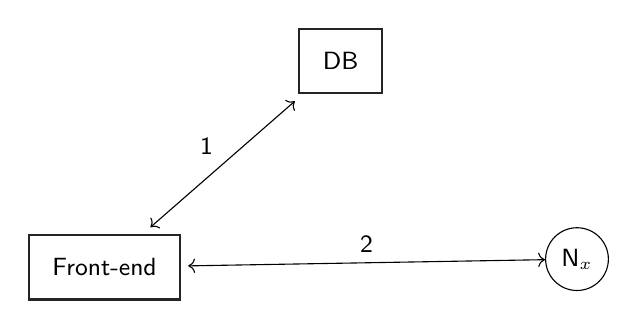
\begin{tikzpicture}
      \node[block] (db) {DB};
      \node[block, below=of db, xshift=-3cm] (fe) {Front-end};
      \node[O, below=of db, xshift=3cm] (Nx) {N$_{x}$};

      \draw[<->] (fe) -- node {1} (db);
      \draw[<->] (fe) -- node {2} (Nx);
    \end{tikzpicture}
  \end{center}
  \caption{
    Repository lookup in database:
    DB --- Database with metadata for current region.
    1 step --- front-end load balancer query database for repository metadata.
    2 step --- front-end access node N$_{x}$ with required repository.
  }\label{fig:repo-lookup-db}
\end{figure}

\begin{figure}
  \begin{center}
    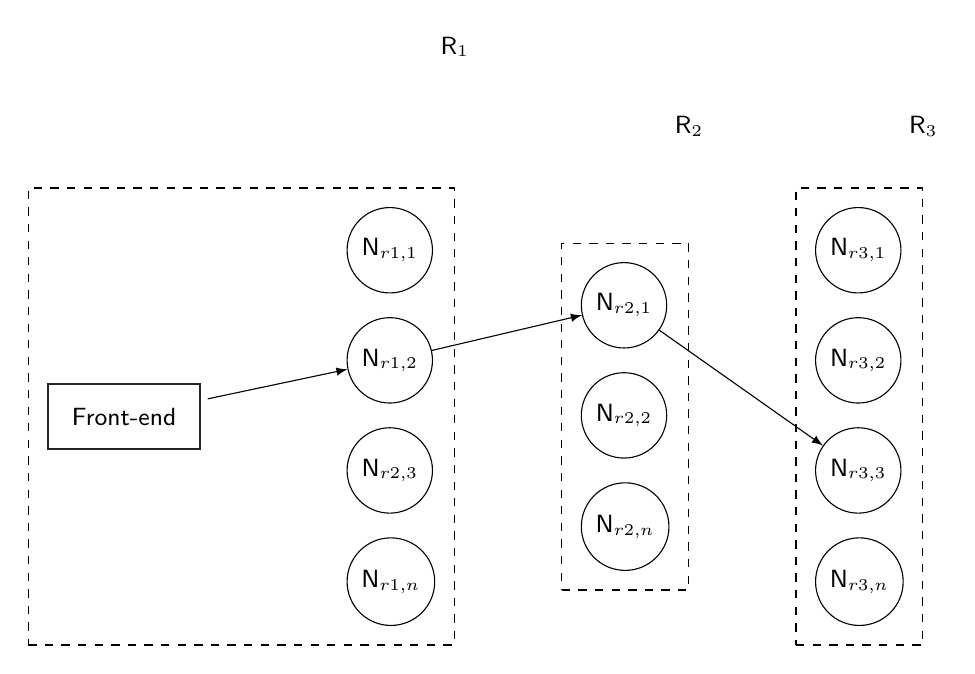
\begin{tikzpicture}
      \matrix[row sep=10mm](feg){
        \node[block] (fe) {Front-end}; \\
      };
      \matrix[row sep=3mm, column sep=5mm, right=of feg](r1){
        \node[O] (r1n1) {N$_{r1,1}$}; \\
        \node[O] (r1n2) {N$_{r1,2}$}; \\
        \node[O] (r1n3) {N$_{r2,3}$}; \\
        \node[O] (r1nN) {N$_{r1,n}$}; \\
      };
      \node[fit=(r1)(feg), draw, dashed, label={[right=0cm, above=3cm]1cm:R$_{1}$}](r1g){};
      \matrix[row sep=3mm, column sep=5mm, right=of r1](r2){
        \node[O] (r2n1) {N$_{r2,1}$}; \\
        \node[O] (r2n2) {N$_{r2,2}$}; \\
        \node[O] (r2nN) {N$_{r2,n}$}; \\
      };
      \node[fit=(r2), draw, dashed, label={[right=0cm, above=3cm]1cm:R$_{2}$}](r2g){};
      \matrix[row sep=3mm, column sep=5mm, right=of r2](r3){
        \node[O] (r3n1) {N$_{r3,1}$}; \\
        \node[O] (r3n2) {N$_{r3,2}$}; \\
        \node[O] (r3n3) {N$_{r3,3}$}; \\
        \node[O] (r3nN) {N$_{r3,n}$}; \\
      };
      \node[fit=(r3), draw, dashed, label={[right=0cm, above=3cm]1cm:R$_{3}$}](r3g){};
      \draw[-latex] (fe) -- (r1n2);
      \draw[-latex] (r1n2) -- (r2n1);
      \draw[-latex] (r2n1) -- (r3n3);
    \end{tikzpicture}
  \end{center}
  \caption{
    Repository lookup via DHT:
    When a front-end in Region R$_{1}$ is unable to find repository located on node N$_{r3,3}$ in same region,
    it queries the nearest known node N$_{r2,1}$. The node N$_{r2,1}$ knows where repository is located
    and redirects the query to node N$_{r3,3}$ with repository.
  }\label{fig:repo-lookup-dht}
\end{figure}

\subsection{Security}\label{subsec:security}

A small fraction of malicious nodes can prevent correct message delivery throughout the overlay.

Such nodes may misroute, corrupt, or drop messages and routing information.
Additionally, they may attempt to assume the identity of other nodes and corrupt or delete objects
they are supposed to store on behalf of the system.

All attacks are based on the presence of malicious nodes.
There are two ways:
\begin{itemize}
  \item[$-$] Implement techniques that allow nodes to join the overlay, maintain routing state, and forward messages securely in malicious nodes.
  \item[$-$] Make the appearance of malicious nodes impossible.
\end{itemize}

Degitx is not an open peer-to-peer system
where resource pooling without preexisting trusted relationships is possible.
It means that untrusted nodes aren't allowed to join
and all members of the network are trusted not to cheat.

To be sure that the node is trusted, its nodeId certificates should be signed by trusted CAs.
Then each node rejects all unsigned requests.

Certified nodeIds work well when nodes have fixed nodeIds.
This condition is met while the node uses a cryptographic hash of public key as nodeId.

These certificates give the overlay a public key infrastructure
suitable for establishing encrypted and authenticated channels between nodes.
Nodes with valid nodeId certificates can join the overlay, route messages,
and repeatedly leave without the involvement of the CAs.

When the membership of a peer-to-peer system is a constraint and all nodes are trusted as in DeGitX (??????),
%FIXME
% CAs could solve security issues, since according to the ~\cite{securerouting} research, all attacks are based on the presence of malicious nodes.

\subsection{Git data exchange}\label{sec:data}

Git is a \href{https://git-scm.com/book/en/v2/Git-Internals-Git-Objects}{content-addressable} file system,
it means that we can safely upload blob objects asynchronously to repository replicas with different changes,
since each blob object will have different name (address) due to content-digest naming.

When multiple clients (front-ends) uploads different changes simultaneously (to different branch or same branch, doesn't matter),
ginternal git storage algorithm guarantee that file names fill be different and correlation is not possible.
The only possible scenario when different clients may upload same blob object is when clients uploads
exactly same changes by all aspects. But in this case it's not a problem, since identical changes will not override
each other, and blob data will be stored consistently.

To summarize --- we allow clients to upload blobs asynchronously to all replicas before uploading references.

The only problem we need to solve is a git references synchronization. We have to update references atomically
on all repository replicas. If any replica fails to update git reference, then the whole reference update should fail.
For this problem we can uses some atomic commit protocol. The possible solutions are three phase commit (3PC), and
two phase commit modification (2PC) with replicas vouting mechanism implemented via total ordering broadcasts,
for example \href{https://www.microsoft.com/en-us/research/uploads/prod/2004/01/twophase-revised.pdf}{Paxos-commit}
could be used. The \href{https://git-scm.com/docs/githooks.html#_reference_transaction}{git reference transaction hook}
will help us to implement a voting for transaction using git.

\todo{update these steps when decide about atomic-commit protocol}.

The overall scenario for updating repository replicas is following:
\begin{enumerate}
    \item The front end uploads git blobs asynchronously to all repository replicas.
    \item On success, the front-end initiates reference update by introducing itslef
      as transaction manager (TM). It sends references update to back-ends (resource managers RM).
    \item RM starts reference update transaction and initiates voting by sending prepare messages
      to all? other RMs.
    \item \todo{add more details}
    \item If all RMs can prepare for transaction, TM sends accept message, and RMs apply references updates
      to repository. If any RM is not able to prepare for the transaction, TM aborts the transaction
      on all RMs.
\end{enumerate}


\section{Special cases}\label{sec:explanation}
\subsection{How to create new repository}

The diagram~\ref{fig:ex-create-repo} explains how administrator creates new repository with replication
on predefined storage nodes by specifying its locator IDs:
\begin{description}
  \item[1] Administrator sends request to the dashboard to create new repository \code{R} at nodes with locators
    \code{L}
  \item[2] Dashboard service performs a lookup of \code{R} in metadata storage
  \item[3] Metadata storage returns locator IDs \code{L'} of \code{R} repository if any
  \item[4, 5] If \code{L'} locators are not emmpty, dashboard returns error to administrator
  \item[6] If no node locator is associated with repository \code{R}, then dashboard asynchronously sends
    requests to each node with locator ID \code{l} from list \code{L}
  \item[7] Dashboard asks node \code{l} to start manage repository \code{R}, and specify other node locator IDs;
    The node \code{l} try to organize consensus between nodes \code{L}, and leader asks all other members
    to manage repository \code{R}
  \item[8] On success, node \code{l} updates metadata with mapping of repository \code{R} hash to
    node locator \code{l}
  \item[9] Meanwhile, the dashboard is performing query requests to the metadata storage to get locator IDs of
    repository \code{R}; Metadata storage returns IDs \code{L'}.
  \item[10] In case if \code{L'} is a subset of \code{L} and the size of \code{L'} is greater or equal to
    half size of \code{L} plus 1 (\code{size(L') >= size(L)/2 + 1})
  \item[11] Dashboard finishes with success status
  \item[12] If waiting timeout is reached
  \item[13] Dashboard finishes with error status
  \item[14] Dashboard returns with success or error status to administrator

\end{description}
\begin{figure}
  \begin{center}
    \begin{tikzpicture}
      \begin{umlseqdiag}
        \umlactor[no ddots]{Administrator}
        \umlcontrol[no ddots]{Dashboard}
        \umlmulti[no ddots]{Nodes}
        \umldatabase[no ddots]{Metadata}

        \begin{umlcall}[op={1: create(R, L)}]{Administrator}{Dashboard}
          \begin{umlcall}[op={2: lookup(R)}]{Dashboard}{Metadata}
            \begin{umlcall}[op={3: L'}, type=return]{Metadata}{Dashboard}
            \end{umlcall}
          \end{umlcall}

          \begin{umlfragment}[type=ALT, name=err-already-exist, inner xsep=3,
            label={4: !empty(L')}]
            \begin{umlcall}[op={5: error}, type=return]{Dashboard}{Administrator}
            \end{umlcall}
            \umlfpart[else]
            \begin{umlfragment}[type=LOOP, inner xsep=7, label={6: for l in L}]
              \begin{umlcall}[op={7: l.manage(R, L)}, type=asynchron]{Dashboard}{Nodes}
                \begin{umlcall}[op={8: update(R, l)}, type=asynchron]{Nodes}{Metadata}
                \end{umlcall}
              \end{umlcall}
            \end{umlfragment}
            \begin{umlfragment}[type=LOOP]
              \begin{umlcall}[op={9: lookup(R)}, return={L'}]{Dashboard}{Metadata}
              \end{umlcall}
              \begin{umlfragment}[type=OPT, label={10: contains(consensus(L), L')}]
                \begin{umlcallself}[op={11: break(success=true)}]{Dashboard}
                \end{umlcallself}
              \end{umlfragment}
              \begin{umlfragment}[type=OPT, label={12: timeout}]
                \begin{umlcallself}[op={13: break(success=false, err=timeout)}]{Dashboard}
                \end{umlcallself}
              \end{umlfragment}
            \end{umlfragment}
            \begin{umlcall}[type=return, op={14: (success, err)}]{Dashboard}{Administrator}
            \end{umlcall}
          \end{umlfragment}
        \end{umlcall}
      \end{umlseqdiag}
    \end{tikzpicture}
  \end{center}
  \caption{Create repository workflow diagram}
  \label{fig:ex-create-repo}
\end{figure}


\subsection{How the node finds the replica with git repository}

Each node (both front-end and back-end nodes) has metadata exchange and discovery protocol components,
both components rely on network modules and locator systems.

Stakeholders:
\begin{description}
  \item[Node] A node which performs repository lookup operation
  \item[RDB] Regional database (caches repository hash table in local region specific cache table)
  \item[DHT] Distributed hash table nodes, can perform global query lookup for node address by repository hash
\end{description}

The legend: \code{r} --- repository hash to lookup; \code{(l, a)} --- repository coordinates,
pair of replica locator IDs and network address, see figure~\ref{fig:ex-node-lookup} for details.

Workflow:
\begin{enumerate}
    \item Node checks local cache populated by local peer discovery broadcasts
      and updated annually after successful query operation
    \item If coordinates were not found in the cache, the node goes to the next lookup layer
    \item Node queries the regional database to find repository coordinates
    \item If coordinates were not found in the database, it goes to the next lookup layer
    \item Node queries DHT nodes using lookup algorithms, e.g., Kademlia.
    \item On success, the node updates the regional database with actual information
    \item Node stores actual information in the local cache
\end{enumerate}

\begin{figure}
  \begin{center}
    \begin{tikzpicture}
      \begin{umlseqdiag}
        \umlobject[no ddots]{Node}
        \umldatabase[no ddots]{RDB}
        \umlmulti[no ddots]{DHT}
        \begin{umlcallself}[op={1: getCache(r)}]{Node}
        \end{umlcallself}
        \begin{umlfragment}[type=OPT, label={2}]
          \begin{umlcall}[op={3: query(r)}, return={(l, a)}]{Node}{RDB}
          \end{umlcall}
          \begin{umlfragment}[type=OPT, label={4}]
            \begin{umlcall}[op={5: query(r)}, return={(l, a)}, dt=7]{Node}{DHT}
            \end{umlcall}
            \begin{umlcall}[op={6: update(r, (l, a))}]{Node}{RDB}
            \end{umlcall}
          \end{umlfragment}
          \begin{umlcallself}[op={7: putCache(r, (l, a))}]{Node}
          \end{umlcallself}
        \end{umlfragment}
      \end{umlseqdiag}
    \end{tikzpicture}
  \end{center}
  \caption{Node discovery and metadata exchange components}
  \label{fig:ex-node-lookup}
\end{figure}

\subsection{How GitLab pushes to DeGitX via Gitaly front-end}

GitLab communicates with DeGitX storage via Gitaly front-end. The front-end
exposes Gitaly gRPC~API.\@ GitLab performs push with two RPC calls:
\begin{description}
  \item[InfoRefsReceivePack] --- to fetch latest repository git references before pushing
  \item[PostReceivePack] --- for add new git objects to the repository
\end{description}

At figure~\ref{fig:gitlab-push-gitaly}, the front-end updates repository lookup routing table
to request git references from one of the replicas and send new git objects to back-end nodes.
See~\ref{sec:appendix-a} to become familiar with git internals.

This diagram explains only communication between GitLab and DeGitX Gitaly front-end.
To understand how the front-end can read and write git data from/to back-ends, see
other diagrams provided below.

\begin{figure}
\centering
  \begin{tikzpicture}
    \begin{umlseqdiag}
      \umlcontrol[no ddots]{git}
      \umlobject[no ddots]{GitLab}
      \umlmulti[no ddots]{DeGitX-FE}
      \umldatabase[no ddots]{Meta}
      \umlmulti[no ddots]{DeGit-BE}
      \begin{umlcall}[op=git-push, return=success]{git}{GitLab}
        \begin{umlcall}[op={InfoRefsReceivePack(R)}]{GitLab}{DeGitX-FE}
          \begin{umlcall}[op={lookup(R)}, return={L}]{DeGitX-FE}{Meta}
          \end{umlcall}
          \begin{umlfragment}[type=ALT, inner xsep=6, label={\code{empty(L)}}]
            \begin{umlcall}[type=return, op={err-not-found}]{DeGitX-FE}{GitLab}
            \end{umlcall}
          \umlfpart[else]
            \begin{umlcallself}[op={\code{update\_cache(R, L)}}]{DeGitX-FE}
            \end{umlcallself}
            \begin{umlcall}[op={L$_{lb}$ \code{read\_refs(R)}}, return={\code{refs}}]{DeGitX-FE}{DeGit-BE}
            \end{umlcall}
            \begin{umlcall}[type=return, op={\code{refs}}]{DeGitX-FE}{GitLab}
            \end{umlcall}
          \end{umlfragment}
        \end{umlcall}
        \begin{umlfragment}[type=OPT, inner xsep=5, label={found}]
          \begin{umlcall}[op={\code{PostReceivePack(R, bin)}},return={success}]{GitLab}{DeGitX-FE}
            \begin{umlcall}[op={L$_{lb}$ \code{receive\_pack(R, bin)}}]{DeGitX-FE}{DeGit-BE}
            \end{umlcall}
          \end{umlcall}
        \end{umlfragment}
      \end{umlcall}
    \end{umlseqdiag}
  \end{tikzpicture}
\caption{%
  User pushes git data to repository \code{R} via Gitlab using \code{git-push} command;%
  Gitlab calls \code{InfoRefsReceivePack} of DeGitX front-end to get latest information%
  about repository \code{R}; front-end perorms lookup in metadata storage,%
  if repository was not found, front-end returns error for gRPC~call;%
  otherwise, it updates local cache with repository locators \code{L}, and reads git references from%
  any load-balanced replica \code{L$_{lb}$}; the front-end returns git data to GitLan server;%
  on success, GitLab sends \code{PostReceivePack} gRPC~call to DeGitX front-end with data to push \code{bin};%
  front-end write data via \code{receive\_pack} git method to any replica \code{L$_{lb}$};%
  (see other examples to understand how back-end nodes updates repository data on push).%
}\label{fig:gitlab-push-gitaly}
\end{figure}

\subsection{How the front-end pushes data to the storage}

The diagram~\ref{fig:ex-push-to-repo} explains how the front-end can push data to the git repository.
Front-end ``FE'' chooses one repository ``R'' replica to communicate with (``BE$_{1}$'' in example diagram),
this node is responsible for talking to the leader or initiate leader election if no leader exists.
The leader is responsible for replicating push command and data across consensus of replicas
and notifying BE$_{1}$ node on success.

On this diagram, the stakeholders are:
\begin{description}
  \item[FE] --- front-end of DeGitX (load-balancer, multiplexer), who received the request to push new data
  \item[BE$_{1}$] --- the back-end of DeGitX (git storage), chosen by front-end load-balancer to interact with
  \item[BE$_{o}$] --- other back-end replicas, containing target repository to push
  \item[Meta] --- Metadata storage (LPD, DB, DHT)
\end{description}

The workflow:
\begin{description}
  \item[1] Client calls RPC of FE to push commits \code{c} to repository \code{r}
  \item[2] FE performs lookup in metadata to find lcoators \code{L[]} of repository \code{r}
  \item[3] FE calls RPC of any storage node from \code{L[]} list to push commits \code{c} to
    repository \code{r}
  \item[4] BE RPC receiver organizes leader-election across replicas of repository \code{r}
    and asks a leader to add new commit \code{c} to repository git storage
  \item[5] At least the half plus one replica performs update and commit new changes
\end{description}

\begin{figure}
  \centering
  \begin{tikzpicture}
    \begin{umlseqdiag}
      \umlobject[no ddots]{FE}
      \umlmulti[no ddots]{BE$_{1}$}
      \umlmulti[no ddots]{BE$_{n}$}
      \umldatabase[no ddots]{Meta}
      \begin{umlcall}[op={lookup(R)}, return={L}]{FE}{Meta}
      \end{umlcall}
      \begin{umlcallself}[op={BE$_{1}$ = any(L)}]{FE}
      \end{umlcallself}
      \begin{umlcall}[op={receive\_pack(R, d)}]{FE}{BE$_{1}$}
        \begin{umlcallself}[op={l = leader(R)}]{BE$_{1}$}
        \end{umlcallself}
        \begin{umlfragment}[type=ALT, name=repl, inner xsep=6, label={l in BE$_{n}$}]
          \begin{umlcall}[op={receive\_pack(R, d)}, return={confirmed}]{BE$_{1}$}{BE$_{n}$}
            \begin{umlcall}[op={append\_entries}]{BE$_{n}$}{BE$_{1}$}
            \end{umlcall}
          \end{umlcall}
        \umlfpart[else]
          \begin{umlcallself}[op={elect}]{BE$_{1}$}
          \end{umlcallself}
          \begin{umlcall}[op={append\_entries}, return={confirmed}]{BE$_{1}$}{BE$_{n}$}
          \end{umlcall}
        \end{umlfragment}
        \umlnote[x=11.5, y=-6.5]{repl}{%
          Add entries to existing leader, or propose itself as leader candidate%
        }
      \end{umlcall}
    \end{umlseqdiag}
  \end{tikzpicture}
  \caption{%
    Front end FE performs query lookup in metadata for repository replicas,%
    chooses any available (BE$_{1}$), and sends \code{receive\_pack} request with pushed data%
    to replica. Replica checks current term leader and asks a leader to add pack to replicated log,%
    in case if leader doesn't exist, the replica initiate new leader election and proposes itself%
    as leader candidate. On success, the replica adds new pack to replicated log via \code{append\_entries}%
    call, and commits the data.%
  }\label{fig:ex-push-to-repo}
\end{figure}

\subsection{How the client fetches git data from repository}

\subsection{How new replica node connected to the cluster}

\todo{explain all questions}


\section{Requirements}
\label{sec:requirements}

\subsection{Features}
\label{sec:features}

The most critical
\href{https://en.wikipedia.org/wiki/Non-functional_requirement}{Non-functional requirements}
are:

\begin{description}
  \item[Read scalability]
    The solution should scale out the read capacity of a system, each region should be able
    to access repository using most available replica node.
  \item[Strong consistency]
    All? (\todo{discuss, maybe not all but the majority of replicas})
    active replica repositories should be synchronized on updates in any node
    with immediate consistency.
  \item[Durability]
    The system must have enough replicas to recover itself in case of corruption.
    Corrupted repository could be responsible for recovering itself using replica nodes.
  \item[Self management (rename?)]
    Each node performs cleanup when needed (\code{git gc}) and may remove replica
    from storage on read inactivity.
    A node should be able to find and synchronize new repository on read,
    after that it should be up to date on new updates.
  \item[Maintainability]
    Node administrator can change the storage, and perform data migration from one storage
    to another.
    Repository administrators are able to add or delete node for new region and
    get all nodes status for repository.
  \item[Auditability]
    Node doesn't perform access control operations, but logs all
    requests with identity and performed operation.
  \item[Analytics]
    Node collects statistics for each repository and usage metrics, such as
    push and pull operations, etc. The system keeps the whole statistics about
    nodes, e.g.\@ how many nodes contains each repository, the state of nodes, etc.
\end{description}

\subsection{Load balancing}\label{sec:load-balancing}

The front-end decides how to redirect incoming fetch requests to replica nodes.
It knows network addresses and current availability of repository replicas,
so it can decide how to route next fetch request to git repository back-end storage node.
On read access to repository, it sends a health check message to replica nodes to be sure
which are available. It stores the result in local cache with configurable time to live
properties. When front-end unable to access some of back-end node, it marks it as unavailable
and forget about it for some time. Then in check availability periodically.
It uses ``Round robin'' load balancing for fetch requests, since it provides uniformly distributed
load for repository nodes on high load peaks. \todo{find references, proves}
Due to strong consistency of back-end nodes provided by data-exchange protocol
it has linearizability property, and provides always latest git data (blobs) and metadata (references).
In case if any node crashes or becomes down, the front-end won't be able to update repository
but it still can read it from live replicas, it means on node failure all repositories located on this
node becomes read-only.

\section{Compare to other solutions}\label{sec:compare}

These products are similar to DeGit by some aspects:
\begin{description}
  \item[Spokes]
    GitHub announced \href{https://github.blog/2016-04-05-introducing-dgit/}{DGit}
    in 2016 (renamed to \href{https://github.blog/2016-09-07-building-resilience-in-spokes/}{Spokes})
    where they \href{https://github.blog/2016-09-07-building-resilience-in-spokes/#defining-resilience}{pay attention}
    to the consistency:
    \begin{quote}
      Spokes puts the highest priority on consistency and partition tolerance.
      In worst-case failure scenarios, it will refuse to accept writes that it cannot commit,
      synchronously, to at least two replicas.
    \end{quote}
    It's a proprietary software that can't be used free and the source code is closed.
    Spokes papers claims that it pays attention to consistency, but on the
    \href{https://www.youtube.com/watch?v=DY0yNRNkYb0}{conference talk} they mentioned that
    it's rarely possible to break the consistency which requires manual intervention.
    Therefore the approach of distributed system design used by Spokes is not suitable for open
    source project, where maintainance team doesn't exist.
  \item[Gitaly]
    \href{https://docs.gitlab.com/ee/README.html}{Gitlab} has
    \href{https://docs.gitlab.com/ee/administration/gitaly/}{Gitaly} service which provides
    \code{gRPC} API for Gitlab website and git-ssh proxy to perform all git operations via API.
    It's \href{https://gitlab.com/gitlab-org/gitaly}{open source} component.
    Gitaly proposed new design for service which claims to provide
    \href{https://gitlab.com/gitlab-org/gitaly/-/blob/master/doc/design\_ha.md\#strong-consistency-design}{strong concistency}
    but in fact it doesn't provide linearability of commands in system \todo{arguments and proves}.
    Futhermore, it's possible that GitLab may change HA licensing \todo{find cases},
    or restrict HA support \href{https://news.ycombinator.com/item?id=21437334}{based on country residence}.
  \item[JGit]
    \href{https://www.eclipse.org/jgit/}{Jgit} is a Java git server created by \href{https://www.eclipse.org/}{Eclipse}.
    Google \href{https://www.eclipse.org//lists/jgit-dev/msg03073.html}{contributed} to this project with Ketch module:
    \begin{quote}
      Git Ketch is a multi-master Git repository management system. Writes
      (such as git push) can be started on any server, at any time. Writes
      are successful only if a majority of participant servers agree.
      Acked writes are durable against server failure, due to a majority of
      the participants storing all required objects.
    \end{quote}
    But this is the only place where Ketch is mentioned. \todo{Analyze source code of Ketch module}.
  \item[IPFS]
    \href{https://ipfs.io/}{IPFS} is not exactly distributed git repository project, but has similar ideas
    and cound be helpfull for us. \todo{analyze IPFS project}.
  \item[brig]
    \todo{analyze the project} \href{https://github.com/sahib/brig}{brig}.
\end{description}

\subsection{Functional Requirements}
\label{sec:nfr}

The most important \href{https://en.wikipedia.org/wiki/Functional_requirement}{functional requirements} are:

\begin{description}
  \item[Front end]
    The system potentically may have different kinds of front-ends,
    but it's required to support \href{https://grpc.io/}{gRPC}
    of \href{https://about.gitlab.com/}{GitLab} to integrate the system
    into GitLab service and replace
    \href{https://docs.gitlab.com/ee/administration/gitaly/}{Gitaly}.
  \item[Back end]
    Each node may be connected to different types of storage for git repos,
    but it's required to support file-system storage.
\end{description}

\subsection{Expected Metrics}
\label{ref:metrics}

In a large enterprise it is expected to have the following
numbers, in terms of load, size, and speed:

\begin{tabular}{ll}
  Repositories & 2M \\
  Active users & 100K/day \\
  Merges & 100K/day \\
  Fetches & 15M/day, 15K/m -- peak \\
  Push & 200K/day \\
  Traffic -- download & 200Tb/day \\
  Traffic -- update & 250Gb/day \\
\end{tabular}

% \include{appendix-a}

\section{References}
\label{ref:references}

Implementing Fault-Tolerant Services Using the State Machine Approach: A Tutorial, FRED B. SCHNEIDER Department of Computer Science, Cornell University, Ithaca, New York 14853 U.S.A.

Replication Management using the State Machine Approach, Fred B. Schneider Department of Computer Science Cornell University Ithaca, NewYork 14853 U.S.A.

Building resilience in Spokes, Patrick Reynolds, https://github.blog/2016-09-07-building-resilience-in-spokes/

Kademlia: A Peer-to-peer information system based on the XOR Metric, Petar Maymounkov and David Mazieres New Yourk University

S/Kademlia: A Practicable Approach Towards Secure Key-Based RoutingIngmar Baumgart and Sebastian MiesInstitute of TelematicsUniversit at Karlsruhe (TH)\@ D–76128 Karlsruhe, Germany

IPFS -- Content Addressed, Versioned, P2P File System (DRAFT 3) Juan Benet

% \printbibliography
\end{document}
